\section{A simple propagation based heuristic for graph clustering}

\subsection*{Prologue}
In this section we come up with a very simple simple clustering
algorithm which uses RWR to divide the well known Zachary's Karate
Club graph. The results can be compared to the actual division of
the subjects of the research into 2 clubs.

\subsection*{Theory}

\begin{mydef}
\label{def:influence}
Let $G$ be a strongly connected graph and $K$ the diffusion matrix as defined in
\ref{lem:invertible}, end let $u,v \in \{1 \dots n\}$ be two vertices and $e_u,
e_v \in \R^n$ their corresponding index vectors.

$p_u := K e_u$, the stationary distribution with random restart from $u$,
is called the \textbf{influence vector} of vertex $u$. We say that
$p_u[v] = K[v,u]$
is the \textbf{influence of} $u$ on $v$. In terms of random walk,
$K[v,u]$ is the frequency that we visit $v$, if we do a RWR from
$u$. 
\end{mydef}

\begin{remark}
\label{rem:influence}
We use the definition of influence as presented in the Hotnet and
Hotnet2 artticles \cite{vandin2012discovery} and
\cite{leiserson2015pan}.

Remember that we use in this paper $A \cdot v$ scheme while
because that is the 'normal' way in linear algebra textbooks.
However often in papers dealing with Markovian processes they use
the other way. To add to the confusion, they sometime call these conventions
left (repectively right) multiplication but whose left and whose
right and why?
\end{remark}

A $p_u$ is a measure of how 'heat' which is pumped into $u$ propagates in the graph.
When we try to cluster the graph, it is natural to think that If vertex $v$
is the top receiver from $u$, namely $v = \text{argmax}(p_u)$ then maybe these 2
belong in the same cluster.

Informally we say that a vertex is 'hot' or 'cold' if it has a high (hot) or low
(cold) PageRank. Remember that the PageRank is the unbiased stationary distribution
$p = K \cdot (1/n, \dots, 1/n)^t$.

We suggest that it makes sense to pick up a
cold vertex and associate it with the vertex to which it sends most of its heat.
If we start from a hot vertex, it usually has many neighbours and it doesn't
send allot of heat down a single vertex.

The algorithm works as follows:

\begin{lstlisting}
function coolWarmClustering(G, k)
  # Input G = (V,E) : a directed strongly connected graph.
  # Input m : The desired number of clusters
  K <- diffusion_kernel(G)
  # each vertex starts in its own cluster: 
  H <- Disconnected_undirected_graph_on(V) 
  p <- pageRank(G)
  # vertex-list sorted up by PageRank: 
  vlist <- arg_sort(p)
  While |connected_components(H)| > k do
    # take the coldest remaining vertex 
    # and remove it from the list:
    x <- vlist.pop()
    # Influence vector of x:
    p_x <-K * e_x 
    # find the max excluding the already visited nodes 
    y <- argmax(p_x[i : i in vlist])
    H.add_edge(x,y)
  return H
\end{lstlisting}

The algorithm clusters the vertices by constructing a new graph on the same
vertices, successively joining vertices. It picks the coldest remaining vertex
and joins it with the vertex to which it propagates the most heat, among
the yet unvisited vertices.

In every iteration of the algorithm adds an edge from the currently
selected vertex to one of the remaining vertices which haven't been
selected yet.The
number of connected components by $1$. Because $G$ is
strongly connected the algorithm will reduce the number of connected
components in $H$ until it reaches the desired number of components
$k$.

It is essential to run the algorith in the order from lower pageranked
vertices upwards. If we start for example the other way around, from
the warmest node downwards, the list of remaining nodes contains the
coldest and least 'relevant' nodes.

\begin{figure}
\begin{framed}
\centering
\begin{subfigure}[b]{0.5\textwidth}
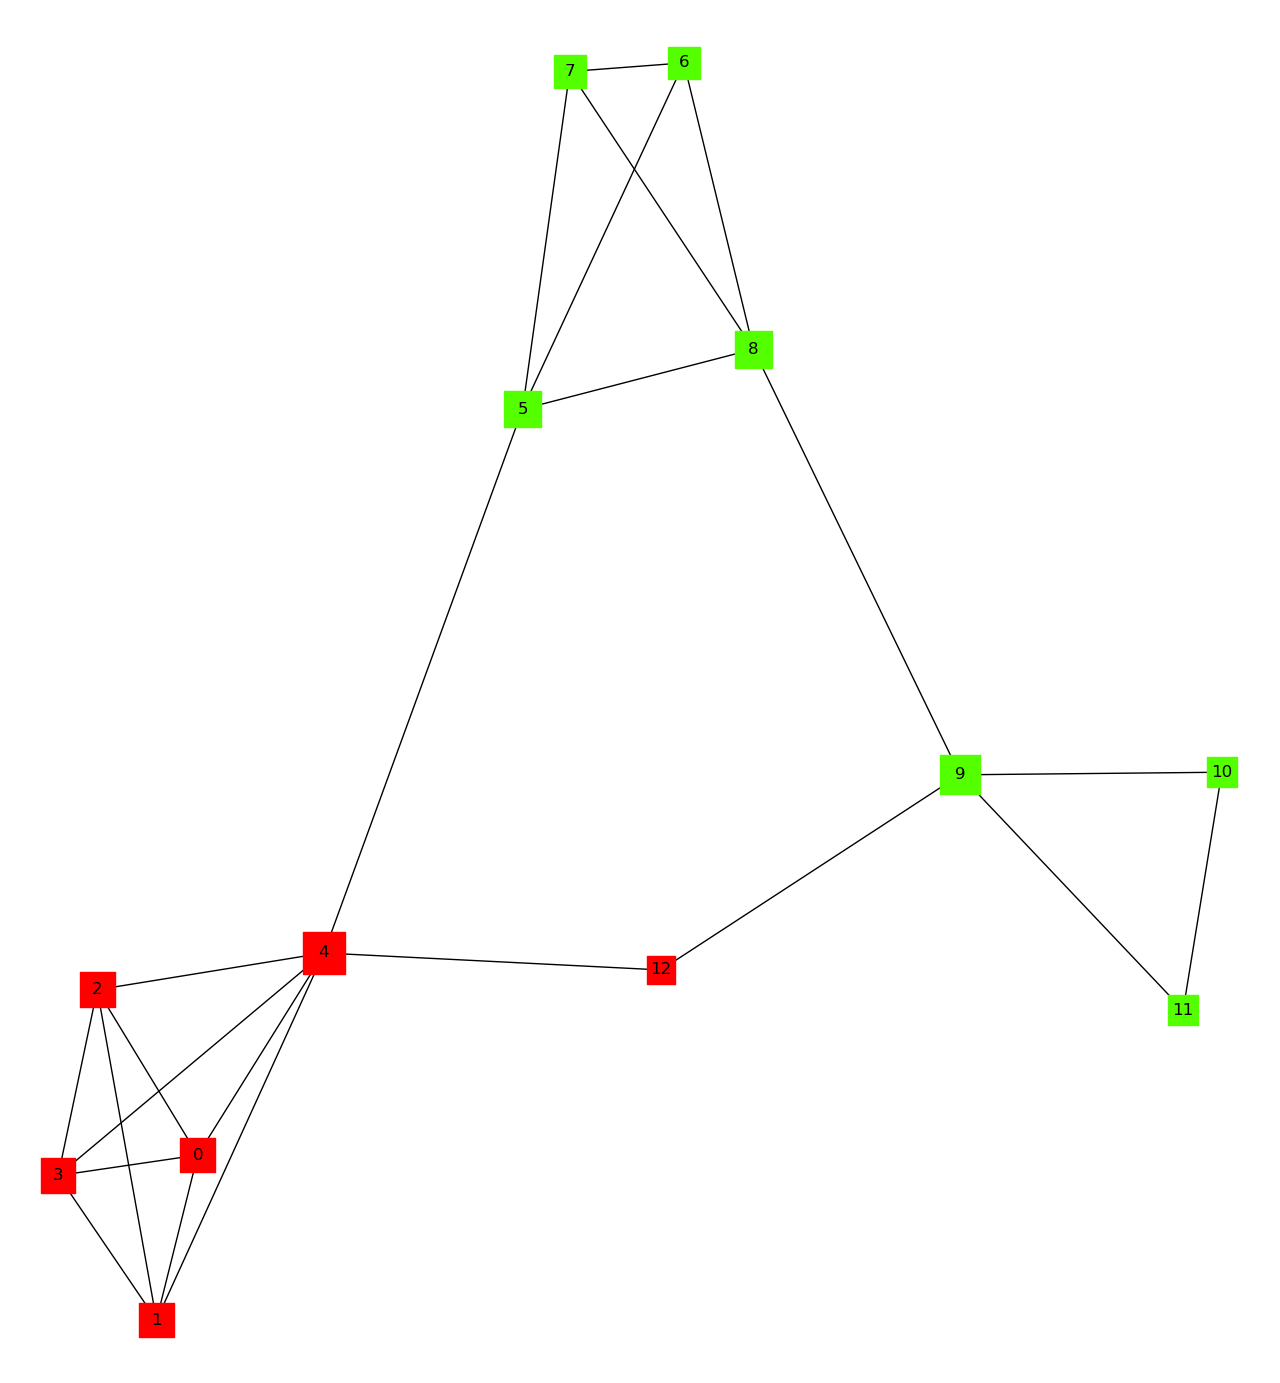
\includegraphics[width=\textwidth]{figures/example_coolwarm2clusters.png}
\caption{A 2 cluster partition}
\label{fig:examplecoolwarm2cluster}
\end{subfigure}
%add desired spacing between images, e. g. ~, \quad, \qquad, \hfill etc. 
%(or a blank line to force the subfigure onto a new line)
\begin{subfigure}[b]{0.5\textwidth}
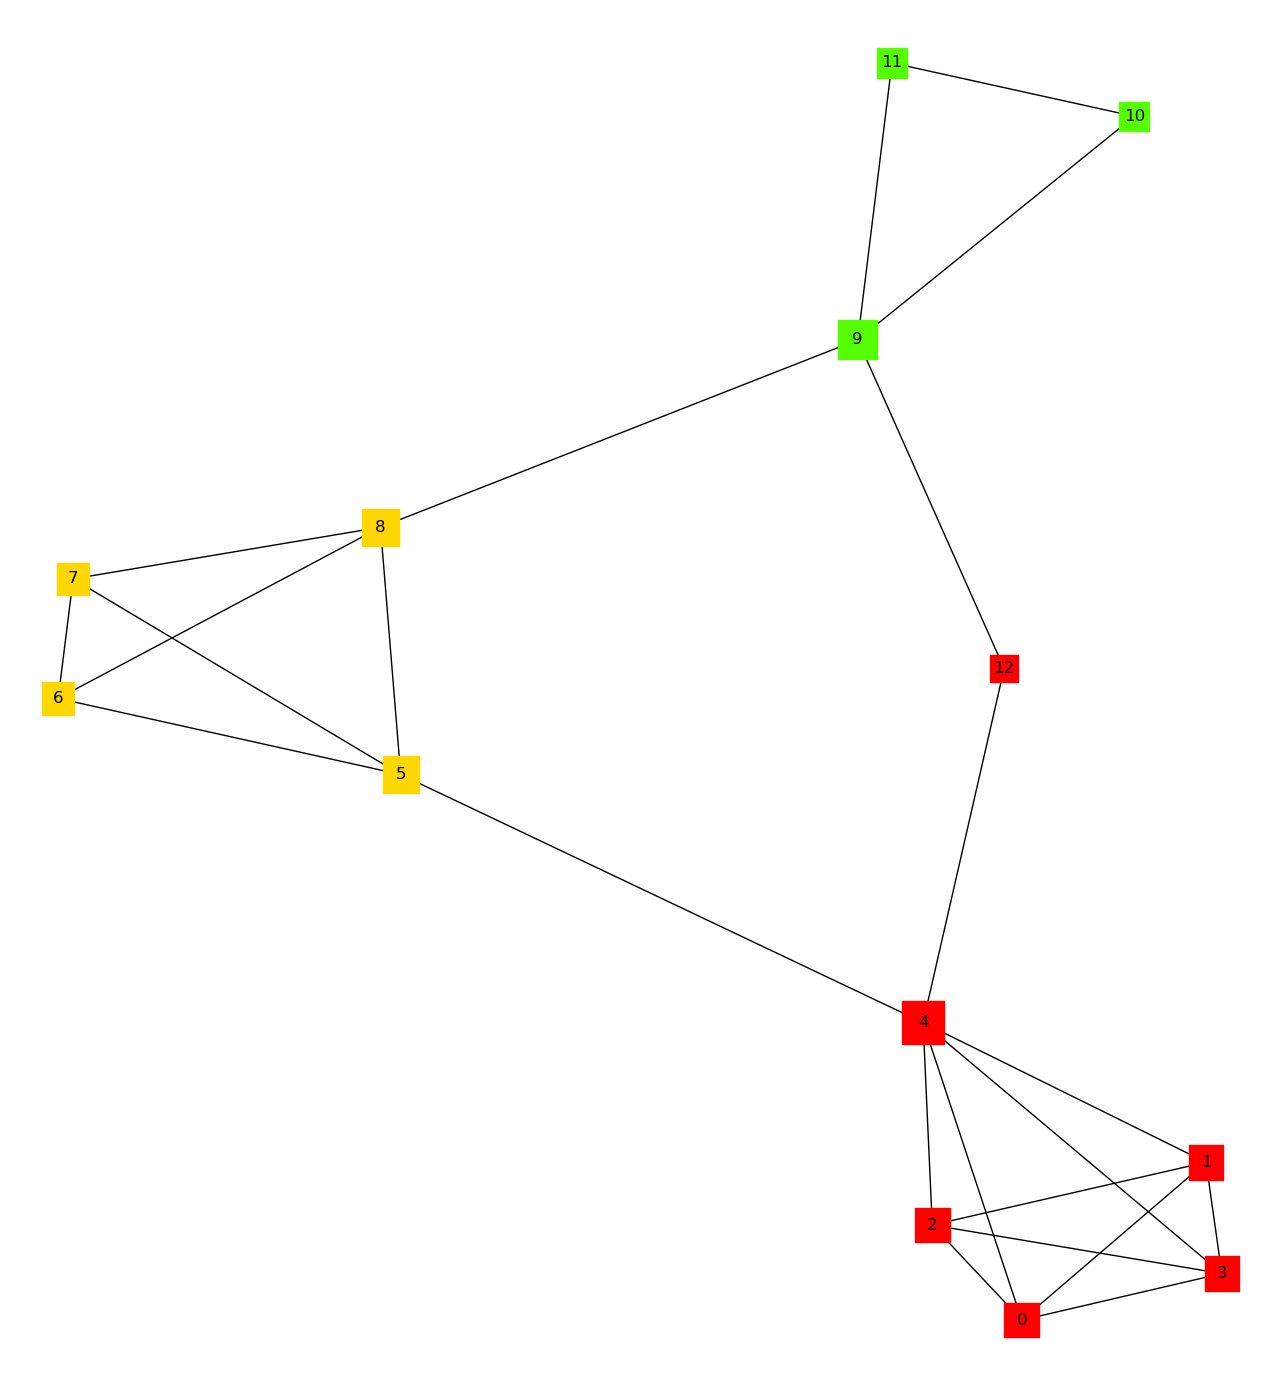
\includegraphics[width=\textwidth]{figures/example_coolwarm3clusters.png}
\caption{A 3 cluster partition}
\label{fig:examplecoolwarm3cluster}
\end{subfigure}
%add desired spacing between images, e. g. ~, \quad, \qquad, \hfill etc. 
%(or a blank line to force the subfigure onto a new line)
\caption{'toy graph' used for testing the algorithm}
\label{fig:exampleCoolWarmClustering}
\end{framed}
\end{figure}

\subsection*{Testing of the algorithm}

We tested the algorithm on a small 'toy graph', as well as on the
famous 'Zachary's Karate Club' graph. In the appendix C, which deals
with spectral clustering, we a tested a basic spectral clustering 
method on the same graphs.

Figures \ref{fig:exampleCoolWarmClustering} are showing the results
of running the algorithm set for finding a 2-partition and
respectively a 3-partition on a 'toy graph'. The interesting node is
12. In both runs 12 chooses to associate with the biggest clique
because node 4 of that clique is the one which receives the most
heat from 12

\begin{figure}[!htb]
\begin{framed}
\centering
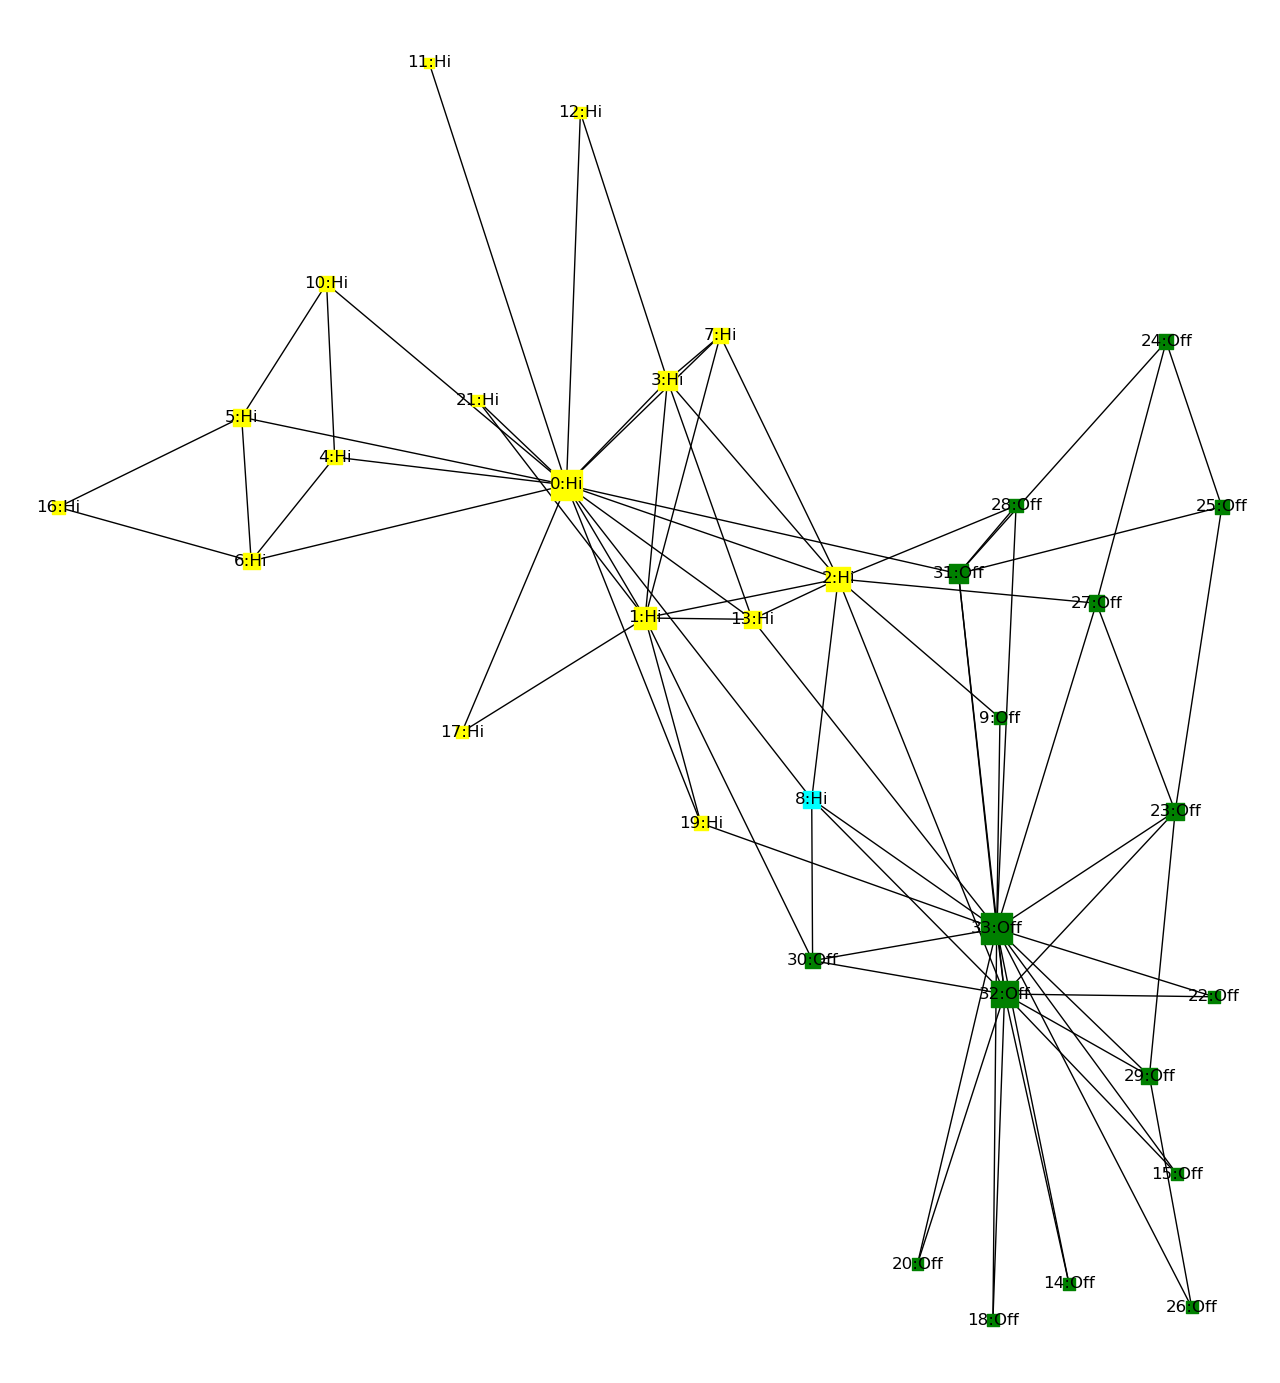
\includegraphics[width=0.75\linewidth]{figures/Karate_coolwarmclustering.png}
\caption{
'Zachary's Karate Club'.
'Mr Hi' (Yellow) and 'Officer' (Green) groups.
The Cyan colored node indicates a mismatch between the clustering
and the actual division.
}
\label{fig:karatecoolwarm}
\end{framed}
\end{figure}

Figure \ref{fig:karatecoolwarm} shows the results of running the
algorithm on the 
famous 'Zachary's Karate Club' Graph. The labels show the actual division
between the 'Mr Hi' and 'Officer' groups.
Vertex size indicates its PageRank.
The colors encode the result of the coolWarmClustering compared to the actual
partition. Yellow indicates true positive for 'Mr Hi', green is a
true positive for 'Officer', and cyan is a mismatch between
the clustering algorithm and the actual division.
There is only one mistake:
It associates wrongly vertex 8 to 'Officer'.  This vertex
is hard to resolve because it is connected to hubs in both clusters.
In fact a further check confirms that the total sum of 'heat' it sends to members of
'Officer' is $0.45$ vs $0.36$ to members of 'Mr Hi' (excluding itself in both
cases). So in some sense the algorithm is more correct then the actual
partition in real life. Perhaps this is due to human irrationality?
On the other hand, vertex $8$ receives more heat units from $17$ members of 'Mr. Hi': $0.485$
units, compared to $0.345$ units from the $16$ members of 'Officer'. 


